\documentclass[mathserif]{beamer}
\usepackage{graphicx}
\usetheme{Frankfurt}
\useinnertheme{rounded}

\title{LEDs for high speed applications \\ (above 100 Mbps)}
\author{Swrangsar Basumatary}
\institute{IIT Bombay, Powai}
\date{April 5, 2013}

    
\begin{document}
    \frame{\titlepage}
    
    \begin{frame}{LEDs vs Laser Diodes for short-range communication}
	    \pause
	    \textbf{Why use LEDs when Laser Diodes are faster?}
            \pause For broadband short-range optical fiber communications, like
LANs and Fiber-in-the-Home networks, LEDs are:
            \pause
            \begin{itemize}[<+->]
                \item cheaper
                \item safer for the human eyes
                \item less sensitive to temperature variations
                \item and more durable
            \end{itemize}
  
        \pause
        \textbf{Disadvantage of using LEDs}
            \begin{itemize}
                \pause \item The problem with LED is \pause \emph{low modulation rate!}\\
                \pause \item While laser diodes have reached to tens of Gbps, \pause 
                commercial DH-LED (double heterostructure) is still limited at 100 Mbps.
            \end{itemize}
        
    \end{frame}
    
    \begin{frame}{Efforts that were not successful}
        \pause
        Efforts have been made to get upto 500 Gbps for conventional LEDs using
        \begin{itemize}
            \pause \item multilevel Pulse Amplitude Modulation (M-PAM)
            \pause \item and discrete multitone modulation (DMT) \\~\\
        \end{itemize} 
        
        \pause But these techniques are \emph{highly complex} compared to the simple on-off keying (OOK) direct modulation scheme.
    \end{frame}
    
    
    
    \begin{frame}{Limitations of OOK modulation rate for LED}
        \pause
        OOK direct modulation rate of LED is limited by two factors:
        
        \begin{enumerate}
            
            \pause \item spontaneous carrier recombination lifetime
            \begin{itemize}
                \pause \item depends on the material and thus it's beyond our control
                \pause \item typically in the range of a few nanoseconds
            \end{itemize}
            
            \pause \item response time (rise time + decay time) of the LED  
            \begin{itemize}
                \pause \item depends on capacitance and dynamic resistance of p-n junctions
                \pause \item \emph{but this can be controlled!} \\~\\
            \end{itemize}
            
        \end{enumerate}
        
        \pause
        So, the only way to increase OOK modulation rate of LED is by \emph{reducing the rise and decay times of the \textbf{EL} signal.}       
    \end{frame}


   
    \begin{frame}{Ways to reduce the response time}
        \pause
        We look at \emph{two} promising ways of improving the response time of the LED have been found upto now
        \begin{enumerate}
            \pause \item using highly-doped InGaAsP/InP Surface Emitting LED with high current density
            \pause \item using Novel LED's driver circuit \\~\\
        \end{enumerate}
        
%        \pause
%        Next, we look at the highly-doped InGaAsP/InP Surface Emitting LED.
    \end{frame}
    
    
    \begin{frame}{Response of an InGaAsP/InP SE LED}
        \pause
        In an undoped InGaAsP/InP Surface Emitting LED
        \begin{itemize}
            \pause \item the rise time decreases with increasing current
            \pause \item but the decay time is higher than the rise time and independent of current
        \end{itemize}
        \pause
 	    \begin{figure}
             \centering
             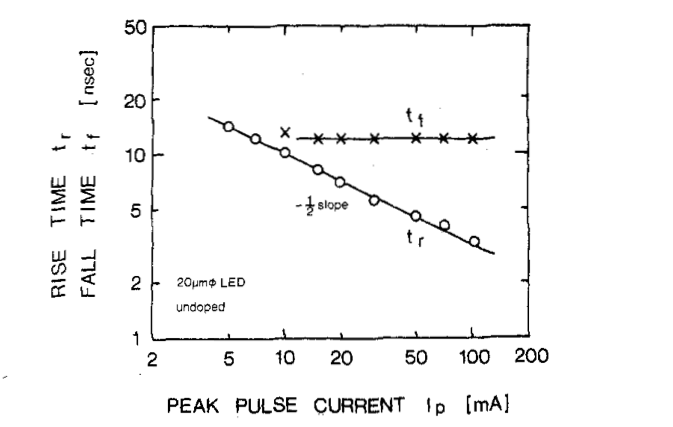
\includegraphics[height=0.4\textheight]{undopedSCLEDResponse.png}
        \end{figure}
%    \end{frame}    
%    \begin{frame}{Response of a heavily doped InGaAsP/InP SE LED}
        \pause
        But with \emph{heavy zinc-doping concentration} in the active layer and low impedance driving circuit the fall time decreases.
%        \pause
% 	    \begin{figure}
%             \centering
%             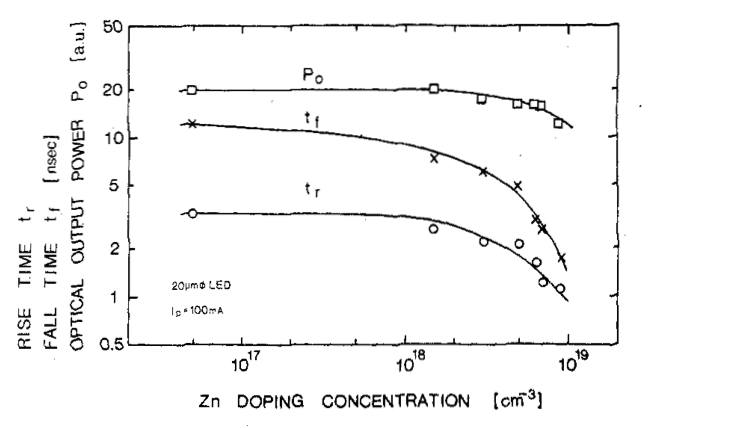
\includegraphics[width=0.8\textwidth]{dopedSCLEDResponse.png}
%        \end{figure}        
    \end{frame}
    
    

	\begin{frame}{Disadvantage of using InGaAsP/InP SE LED}
        \pause A 2 Gbps NRZ pulse transmission over a 500-m span has been carried out using heavy zinc-doped InGaAsP/InP Surface Emitting LED. \\~\\
        \pause But the internal quantum efficiency and thereby overall efficiency of the InGaAsP/InP LED is low. \\~\\
        \pause A better option is to use Novel LED's driver circuit with a relatively lower speed.
    \end{frame}
    
    
    \begin{frame}{LED's Novel Driver Circuit}
        \pause In order to reduce the effect of the LED's diffusion capacitance, this newly proposed driver circuit uses
        \begin{itemize}
            \pause \item \emph{carrier sweep-out effect} in the active region when electrical pulse is turned off
            \pause \item \emph{peaking effect} when electrical pulse is on
        \end{itemize}
        Thus, using this driver circuit we can transmit OOK signal with speed upto 500 Mbps.  
%    \end{frame}
        
    
%    \begin{frame}{Peaking effect and sweep-out effect}
 	    \pause
        \begin{figure}
             \centering
             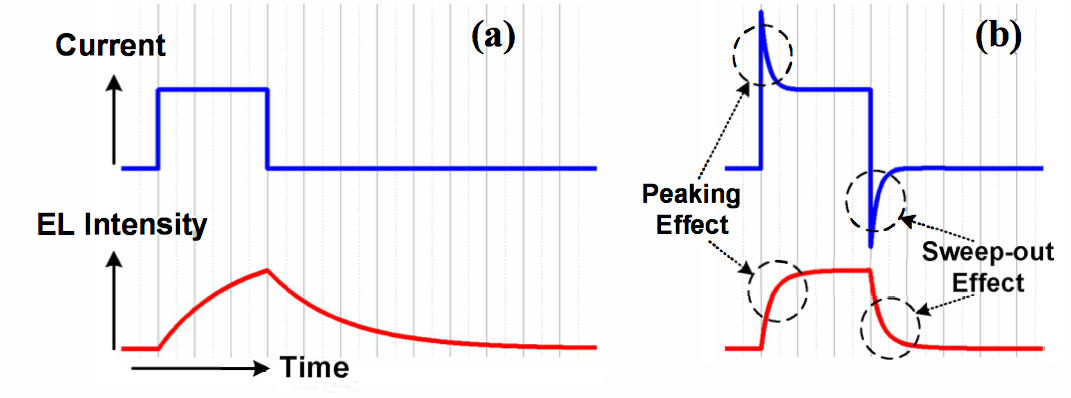
\includegraphics[width=0.8\textwidth]{peakingAndSweepOut.png}
             \caption{(a) EL pulse excited by current pulse. (b) Peaking effect and sweep-out effect}
        \end{figure}
    \end{frame}
    
    
    \begin{frame}{The novel LED driver}
        \pause
        The novel driver uses two Schottky diodes in parallel with a capacitor (SD-C circuit) instead of an RC circuit, as its current-shaping circuit.
        \pause
        \begin{figure}
            \centering
            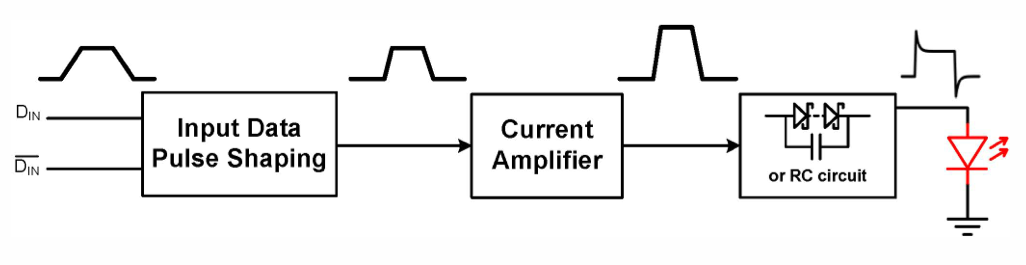
\includegraphics[width=0.8\textwidth]{novelLEDDriver.png}
            \caption{Proposed novel LED driver diagram}
        \end{figure}
    \end{frame}


    \begin{frame}{SD-C circuit vs RC circuit}
        \pause
        The peaking and sweep-out effect are much stronger when using an SD-C circuit than when using an RC circuit.
        \pause
        \begin{figure}
            \centering
            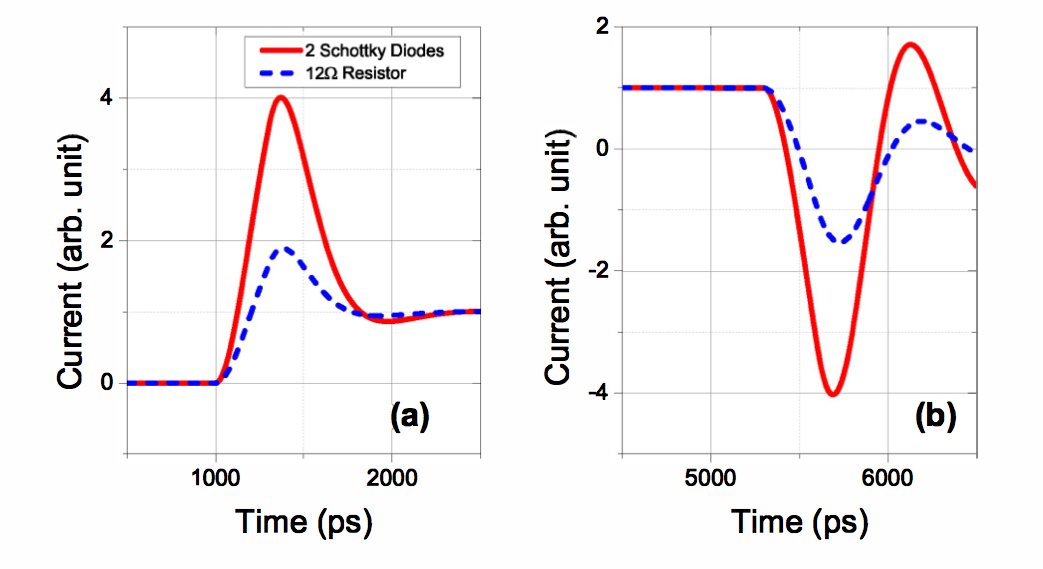
\includegraphics[width=0.8\textwidth]{peakingSweepOutSimulation.png}
            \caption{Simulation of (a) peaking current (b) reverse current of LED in SD-C and RC circuits. Parallel capacitors are 22 pF. Excitation pulse is 3 $V_{p-p}$, rise and fall times of 300 ps.}
        \end{figure}
    \end{frame}


    \begin{frame}{Experimental results}
        \pause
        \begin{figure}
            \centering
            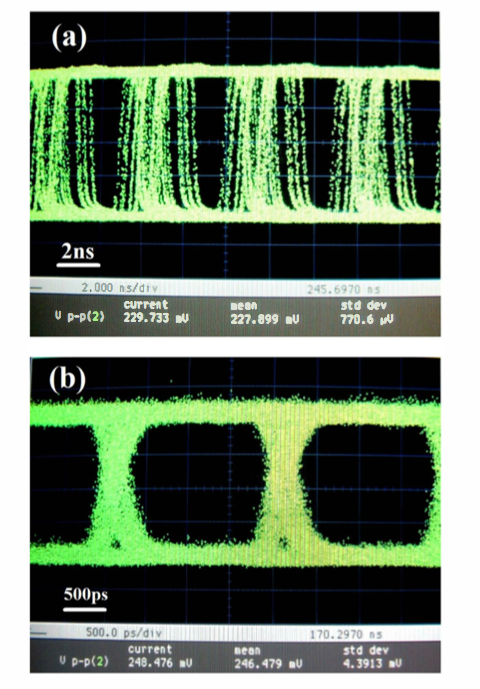
\includegraphics[height=0.6\textheight]{eyeDiagrams.png}
            \caption{Optical eye diagrams using MC2042-4 with (a) RC circuit at 200 Mbps (b) SD-C circuit at 500 Mbps}
        \end{figure}
    \end{frame}
    
    \begin{frame}{References}
        \pause
        \begin{itemize}
                 \item P. H. Binh, V. D. Trong, C.T. Anh, P. Renucci, X. Marie, C. T. Truong, A. T. Pham, ``Novel LED's Driver Circuit for Broadband Short-Range Optical Fiber Communication Systems,'' \emph{Communications and Electronics (ICCE), 2012 Fourth International Conference on}.
                 \item Akira Suzuki, Toshio Uji, Yasumasa Inomoto, Junji Hayashi, Yoichi Isoda, and Hidenori Nomura, ``InGaAsP/InP 1.3-$\mu$m Wavelength Surface-Emitting LED's for High-Speed Short-Haul Optical Communication Systems,'' \emph{IEEE Transactions on Electron Devices}, December 1985.
        \end{itemize}
    \end{frame}
    
    
\end{document}